\documentclass{standalone}
\usepackage{times}
\usepackage{mathtools}
\usepackage{amsfonts}
\usepackage{amssymb}

\usepackage{tikz}
\usetikzlibrary{positioning,fit,shapes,calc,decorations.pathreplacing}
\usetikzlibrary{backgrounds}
\usetikzlibrary{arrows.meta}
\usetikzlibrary{shapes,snakes}

\definecolor{processblue}{cmyk}{1,1,1,0}
\definecolor{accent}{rgb}{0.0,0.5,0.8}
\definecolor{accent2}{rgb}{0.8,0.5,0.0}

\begin{document}
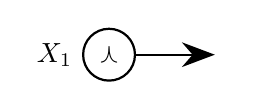
\begin{tikzpicture}[
  node/.style = {
    draw,
    circle,
    thick,
    fill = white,
    minimum width = 0.5cm,
    minimum height = 0.5cm,
  },
  >={Stealth[scale=1.8]},
]

  \node[node] (unit) [label={left:$X_1$}] {$\curlywedge$};
  \node (h) [right=of unit] {};
  \path[->,thick] (unit) edge[out=0,in=180] node {} (h);

\end{tikzpicture}
\end{document}
